% ==================== CHƯƠNG 8 ====================
\newpage
\chap{Thành phần hệ hỗ trợ quyết định (DSS)}\label{sec:dss}

\sect{Quyết định cần hỗ trợ}
Theo nguyên tắc thiết kế DSS (mục~\ref{sec:theory-dss}), nhóm xuất phát từ quyết định cần hỗ trợ:
\begin{itemize}
    \item \textbf{Người ra quyết định}: quản lý vận hành hệ thống xe đạp công cộng.
    \item \textbf{Quyết định}: với một ngày sắp tới (biết trước loại ngày và dự báo thời tiết), mỗi khung giờ cần chuẩn bị nguồn lực ở mức nào - cơ bản, theo dõi, hay tăng cường; khung giờ nào cần ưu tiên và phải sẵn sàng từ lúc nào.
    \item \textbf{Tần suất}: hằng ngày, lặp lại - phù hợp để hỗ trợ bằng hệ thống.
    \item \textbf{Thông tin cần}: nhu cầu lịch sử theo giờ trong các điều kiện tương tự, lấy từ kho dữ liệu.
    \item \textbf{Ràng buộc}: dữ liệu không có số xe sẵn sàng hay vị trí trạm, nên DSS khuyến nghị \textbf{mức độ} chuẩn bị chứ không tính số xe cụ thể; quyết định cuối cùng vẫn do người vận hành đưa ra.
\end{itemize}

\sect{Áp dụng mô hình ra quyết định của Simon}\label{sec:dss-simon}
\begin{table}[H]
\centering
\caption{Bốn giai đoạn ra quyết định và chức năng DSS tương ứng}
\label{tab:simon}
\begin{tabularx}{\textwidth}{|p{2.6cm}|X|X|}
\hline
\textbf{Giai đoạn} & \textbf{Nội dung trong bài toán} & \textbf{Hệ thống hỗ trợ} \\ \hline
Tìm hiểu (Intelligence) & Nhận diện vấn đề thiếu/dư xe theo giờ; tìm hiểu quy luật nhu cầu & Kho dữ liệu, KPI, OLAP, dashboard phân tích (mục~\ref{sec:impl}, \ref{sec:results}) \\ \hline
Thiết kế (Design) & Xây dựng mô hình phân loại nhu cầu, xác định tiêu chí (ngưỡng) và các phương án chuẩn bị & Khảo sát phân phối, quy tắc ra quyết định 3 mức (mục~\ref{sec:dss-model}--\ref{sec:dss-rules}) \\ \hline
Lựa chọn (Choice) & Với tình huống sắp tới, chọn mức chuẩn bị cho từng giờ; xem xét độ nhạy của ngưỡng & Kế hoạch 24 giờ, cảnh báo, danh sách ưu tiên, đổi ngưỡng P33/P67 $\leftrightarrow$ P25/P75, đổi kỳ lịch sử (mục~\ref{sec:dss-results}, \ref{sec:dss-sensitivity}) \\ \hline
Thực hiện (Implementation) & Bố trí xe, nhân sự theo kế hoạch; theo dõi thực tế & Khuyến nghị cụ thể theo mức, giờ cần chuẩn bị xong; dữ liệu mới nạp vào kho để vòng sau cập nhật ngưỡng \\ \hline
\end{tabularx}
\end{table}

\sect{Kiến trúc thành phần DSS}\label{sec:dss-arch}
DSS được tổ chức theo bốn thành phần kinh điển~\cite{turban}:
\begin{itemize}
    \item \textbf{Quản lý dữ liệu}: kho \code{dw}; truy xuất qua \code{src/api/dss\_queries.py} - chỉ lọc theo \textbf{kỳ lịch sử} (năm, mùa, tháng).
    \item \textbf{Quản lý mô hình}: \code{src/dss/engine.py} - Python thuần, không phụ thuộc CSDL, gồm tính ngưỡng, phân loại, gán khuyến nghị, gộp khung cảnh báo, đánh giá độ tin cậy.
    \item \textbf{Tri thức}: bảng quy tắc ra quyết định (mức $\rightarrow$ khuyến nghị) và các hằng số được ghi rõ (\code{MIN\_OBS = 30}, phân vị mặc định).
    \item \textbf{Giao diện}: khu vực ``Hệ hỗ trợ quyết định'' trên dashboard (\code{DssPanel.jsx}) và 3 endpoint \code{/api/dss/thresholds}, \code{/api/dss/plan}, \code{/api/dss/matrix}.
\end{itemize}
Quy trình xử lý gồm 5 bước theo yêu cầu đề tài: (1) người dùng chọn kỳ lịch sử; (2) hệ thống truy xuất dữ liệu từ kho; (3) tính lượt thuê trung bình theo giờ, loại ngày và thời tiết; (4) phân loại thành ba mức; (5) đưa ra khuyến nghị, cảnh báo.

\sect{Mô hình ra quyết định}\label{sec:dss-model}
\subsect{Các biến của mô hình}
\begin{table}[H]
\centering
\caption{Các nhóm biến trong mô hình DSS}
\label{tab:dss-vars}
\begin{tabularx}{\textwidth}{|p{3.6cm}|X|}
\hline
\textbf{Nhóm biến} & \textbf{Biến trong đề tài} \\ \hline
Biến không kiểm soát (tham số tình huống) & Giờ $h \in \{0..23\}$; loại ngày $d \in$ \{làm việc, nghỉ\} hoặc một / nhiều thứ cụ thể trong tuần (thứ hai \ldots{} chủ nhật, không gồm ngày lễ); thời tiết dự kiến $w \in \{1..4\}$; kỳ lịch sử $P$ (năm, mùa, tháng) \\ \hline
Tham số mô hình & Phân vị ngưỡng $q_L, q_H$ (mặc định $1/3$, $2/3$); ngưỡng số mẫu tối thiểu $n_{min} = 30$ \\ \hline
Biến kết quả & Nhu cầu kỳ vọng $\bar{y}_{h,d,w}$; mức nhu cầu \{Thấp, Trung bình, Cao\}; khung cảnh báo; danh sách giờ ưu tiên; tỷ lệ khách vãng lai $c_{h,d,w}$ và nhóm khách \{chủ yếu đăng ký, hỗn hợp, nhiều vãng lai\} \\ \hline
Biến quyết định (người dùng chọn) & Mức chuẩn bị nguồn lực cho từng giờ: cơ bản / theo dõi / tăng cường; loại hỗ trợ: ưu tiên đủ xe đúng giờ / hướng dẫn và hỗ trợ khách mới \\ \hline
\end{tabularx}
\end{table}

\subsect{Công thức}
Gọi $H(P)$ là tập các giờ quan sát trong kỳ lịch sử $P$ và $y_i$ là \code{total\_cnt} của giờ $i$. Nhu cầu kỳ vọng của một nhóm là trung bình của các giờ quan sát cùng giờ, cùng loại ngày, cùng thời tiết:
\[
\bar{y}_{h,d,w} = \frac{1}{n_{h,d,w}} \sum_{i \in H(P),\ hour(i)=h,\ day(i)=d,\ weather(i)=w} y_i
\]
Ngưỡng phân loại là các phân vị của phân phối lượt thuê theo giờ trong kỳ (tính bằng \code{percentile\_cont} của PostgreSQL, nội suy tuyến tính):
\[
\theta_L = Q_{q_L}\big(\{y_i\}_{i \in H(P)}\big), \qquad \theta_H = Q_{q_H}\big(\{y_i\}_{i \in H(P)}\big)
\]
Hàm phân loại:
\[
\text{level}(h,d,w) =
\begin{cases}
\text{Thấp} & \text{nếu } \bar{y}_{h,d,w} < \theta_L \\
\text{Trung bình} & \text{nếu } \theta_L \le \bar{y}_{h,d,w} \le \theta_H \\
\text{Cao} & \text{nếu } \bar{y}_{h,d,w} > \theta_H \\
\text{Không có dữ liệu} & \text{nếu } n_{h,d,w} = 0
\end{cases}
\]

\subsect{Lý do chọn ngưỡng theo phân vị}
\begin{itemize}
    \item Phân phối lượt thuê \textbf{lệch phải mạnh} (trung bình 189,5 $>$ trung vị 142; độ lệch chuẩn 181,4 gần bằng trung bình). Ngưỡng dạng ``trung bình $\pm$ độ lệch chuẩn'' cho cận dưới gần 0 và cận trên 371, phân loại rất mất cân đối. Phân vị không phụ thuộc giả định phân phối chuẩn và bền vững với giá trị ngoại lai.
    \item Tam phân vị chia số giờ quan sát thành ba phần xấp xỉ bằng nhau, nên ý nghĩa của mức rất trực quan: ``Cao'' là nhu cầu thuộc nhóm một phần ba giờ bận rộn nhất trong lịch sử.
    \item Ngưỡng được tính lại theo \textbf{kỳ lịch sử người dùng chọn}, nên tự thích nghi với tăng trưởng: kỳ 2011 có ngưỡng 55/174, kỳ 2012 là 98/284 lượt/giờ.
    \item Ngưỡng là tham số, có thể đổi (P25/P75) để phân tích độ nhạy (mục~\ref{sec:dss-sensitivity}).
\end{itemize}

\sect{Khảo sát phân phối và xác định ngưỡng}
Theo yêu cầu đề tài, ngưỡng phải được xác định \textbf{sau khi khảo sát phân phối dữ liệu}. Hình~\ref{fig:dss-dist} và Bảng~\ref{tab:percentiles} là kết quả khảo sát trên toàn bộ 17.379 giờ quan sát.

\begin{figure}[H]
\centering
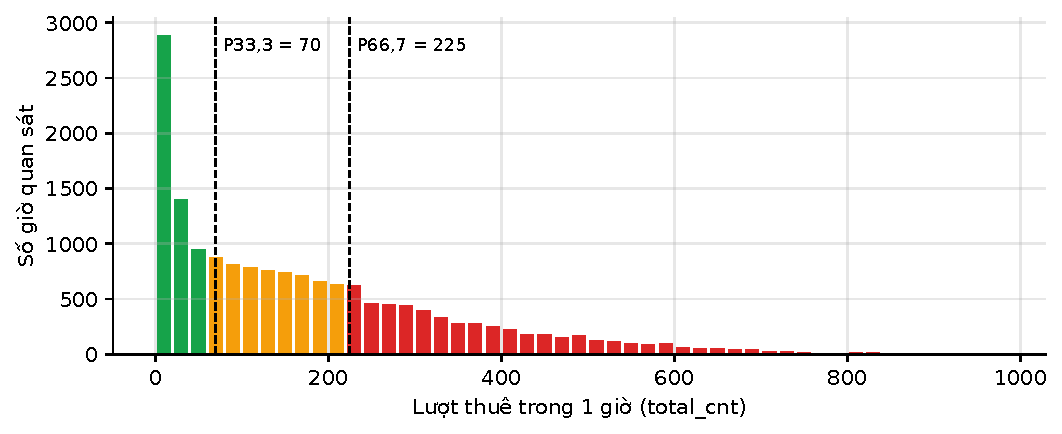
\includegraphics[width=0.95\textwidth]{figures/dss_distribution.pdf}
\caption{Phân phối lượt thuê theo giờ và hai ngưỡng phân loại}
\label{fig:dss-dist}
\end{figure}

\begin{table}[H]
\centering
\caption{Các phân vị của lượt thuê theo giờ (toàn bộ dữ liệu)}
\label{tab:percentiles}
\begin{tabular}{|c|c|c|c|c|c|c|c|c|}
\hline
\textbf{P10} & \textbf{P25} & \textbf{P33,3} & \textbf{P50} & \textbf{P66,7} & \textbf{P75} & \textbf{P90} & \textbf{TB} & \textbf{ĐLC} \\ \hline
9 & 40 & \textbf{70} & 142 & \textbf{225} & 281 & 451 & 189,5 & 181,4 \\ \hline
\end{tabular}
\end{table}
Với $\theta_L = 70$ và $\theta_H = 225$, tỷ lệ giờ quan sát rơi vào ba mức lần lượt là 33,1\%, 33,8\% và 33,1\% - đúng với mục tiêu chia đều.

\sect{Quy tắc ra quyết định và khuyến nghị}\label{sec:dss-rules}
\begin{table}[H]
\centering
\caption{Quy tắc ra quyết định (ngưỡng tính trên toàn bộ dữ liệu)}
\label{tab:rules}
\begin{tabularx}{\textwidth}{|c|p{3.2cm}|X|}
\hline
\textbf{Mức} & \textbf{Điều kiện} & \textbf{Khuyến nghị} \\ \hline
\Low & $\bar{y} < 70$ lượt/giờ & Duy trì mức chuẩn bị cơ bản. Có thể tận dụng khung giờ này để bảo trì, sửa chữa xe. \\ \hline
\Med & $70 \le \bar{y} \le 225$ & Theo dõi nhu cầu và duy trì nguồn lực phù hợp, sẵn sàng bổ sung nếu nhu cầu tăng. \\ \hline
\High & $\bar{y} > 225$ & Ưu tiên chuẩn bị thêm xe và nguồn lực phục vụ (nhân sự điều phối, hỗ trợ) trước khung giờ này. \\ \hline
-- & $n = 0$ & Không có dữ liệu lịch sử cho tình huống này, không đủ căn cứ để khuyến nghị. \\ \hline
\end{tabularx}
\end{table}

\subsect{Cảnh báo và danh sách ưu tiên}
Để trả lời câu hỏi ``khi nhu cầu dự kiến tăng cao, hệ thống cảnh báo gì'' (Q3.4), các giờ liên tiếp ở mức Cao được \textbf{gộp thành một khung cảnh báo}. Mỗi cảnh báo nêu: khoảng thời gian, giờ đỉnh và nhu cầu trung bình tại đỉnh, \textbf{thời điểm phải hoàn tất chuẩn bị} (một giờ trước khi khung bắt đầu). Các giờ Cao được sắp xếp giảm dần theo nhu cầu tạo thành \textbf{danh sách ưu tiên} (Q3.1). Ngoài ra, mỗi giờ có chỉ số \textit{so với trung bình kỳ} ($\bar{y}_{h,d,w} / \bar{y}$) để người vận hành hiểu mức độ chênh lệch.

\subsect{Nhóm khách cần phục vụ}\label{sec:dss-users}
Dữ liệu tách lượt thuê thành hai nhóm: \textbf{khách đăng ký} (thành viên, chủ yếu đi làm, đi học) và \textbf{khách vãng lai} (thuê lẻ, chủ yếu đi chơi, tham quan). Nhóm cân nhắc hai cách đưa thông tin này vào DSS:
\begin{itemize}
    \item \textit{Xếp mức riêng cho từng nhóm} (ngưỡng tính trên phân phối của nhóm đó): với khách vãng lai, ngưỡng Cao chỉ là 34 lượt/giờ nên gần như cả ban ngày (10--20h ngày làm việc, 9--21h ngày nghỉ) đều thành Cao - khuyến nghị mất khả năng phân biệt; với khách đăng ký (81\% lượt thuê), kết quả gần như trùng với cách xếp theo tổng.
    \item \textit{Giữ mức theo tổng, bổ sung thành phần khách} (\textbf{cách được chọn}): xe là tài sản dùng chung cho cả hai nhóm nên \textbf{số xe cần chuẩn bị} phụ thuộc tổng lượt thuê; còn \textbf{thành phần khách} quyết định \textbf{loại hỗ trợ} cần bố trí.
\end{itemize}
Gọi $c_{h,d,w}$ là tỷ lệ khách vãng lai của nhóm (tổng lượt vãng lai trung bình chia tổng lượt trung bình) và $\bar{c}$ là tỷ lệ vãng lai chung của kỳ lịch sử ($\bar{c} = 18{,}8\%$ trên toàn bộ dữ liệu). Mốc phân nhóm được đặt tương đối so với $\bar{c}$ nên tự điều chỉnh theo kỳ được chọn:
\[
\text{segment}(h,d,w) =
\begin{cases}
\text{Nhiều khách vãng lai} & \text{nếu } c_{h,d,w} \ge 1{,}5\,\bar{c} \quad (\ge 28{,}2\%)\\
\text{Chủ yếu khách đăng ký} & \text{nếu } c_{h,d,w} \le 0{,}75\,\bar{c} \quad (\le 14{,}1\%)\\
\text{Khách hỗn hợp} & \text{còn lại}
\end{cases}
\]
Tỷ lệ của một khung cảnh báo được tính có trọng số theo lượt thuê ($\sum$ vãng lai $/ \sum$ tổng của các giờ trong khung). Mỗi nhóm khách có một khuyến nghị bổ sung: \textit{chủ yếu đăng ký} - ưu tiên có đủ xe sẵn sàng đúng giờ, điều phối xe kịp thời; \textit{nhiều vãng lai} - bố trí nhân sự hướng dẫn thuê xe, hỗ trợ thanh toán và giải đáp cho khách mới; \textit{hỗn hợp} - kết hợp cả hai. Khuyến nghị này được ghép vào nội dung cảnh báo của khung.

\begin{lstlisting}[language=Python, caption={Phân loại và gộp khung cảnh báo (trích \code{src/dss/engine.py})}]
def classify(value, th):
    if value is None:
        return None                 # no historical data
    if value < th["low"]:
        return "low"
    if value > th["high"]:
        return "high"
    return "medium"

def high_windows(hours):            # hours: 24 items sorted by hour
    windows, cur = [], None
    for h in hours:
        if h["level"] == "high":
            if cur and h["hour"] == cur["end_hour"] + 1:
                cur["end_hour"] = h["hour"]; cur["hours"].append(h)
            else:
                cur = {"start_hour": h["hour"], "end_hour": h["hour"], "hours": [h]}
                windows.append(cur)
        else:
            cur = None
    return windows                  # + peak hour, prepare_before = start - 1
\end{lstlisting}

\subsect{Độ tin cậy}
Nhóm có ít hơn $n_{min} = 30$ giờ quan sát được gắn cờ \textit{độ tin cậy thấp} (hiển thị nhạt trên giao diện, kèm ghi chú); nhóm không có quan sát nào không được phân loại. Đây là cách DSS xử lý trung thực vấn đề dữ liệu thưa: mức thời tiết 4 chỉ có 3 giờ quan sát nên kịch bản ``ngày nghỉ, mưa lớn'' có 23/24 giờ không có dữ liệu, và hệ thống nói rõ điều đó thay vì suy diễn.

\sect{Kết quả của DSS}\label{sec:dss-results}
Hình~\ref{fig:dss-plan} là kế hoạch 24 giờ cho hai tình huống thường gặp nhất. Bảng~\ref{tab:scenarios} tóm tắt kết quả cho sáu tình huống có đủ dữ liệu.

\begin{figure}[H]
\centering
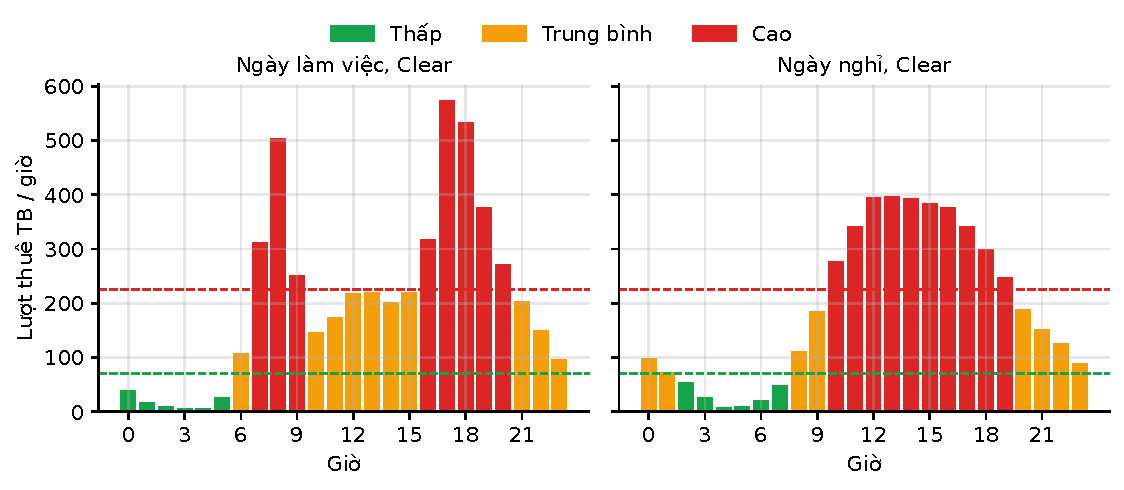
\includegraphics[width=\textwidth]{figures/dss_plan.pdf}
\caption{Mức nhu cầu dự kiến theo giờ: ngày làm việc và ngày nghỉ, trời quang (đường nét đứt: ngưỡng 70 và 225)}
\label{fig:dss-plan}
\end{figure}

\begin{table}[H]
\centering
\caption{Kết quả DSS theo tình huống (ngưỡng P33,3/P66,7, toàn bộ dữ liệu)}
\label{tab:scenarios}
\small
\begin{tabularx}{\textwidth}{|l|l|c|c|c|X|p{2.6cm}|}
\hline
\textbf{Loại ngày} & \textbf{Thời tiết} & \textbf{Thấp} & \textbf{TB} & \textbf{Cao} & \textbf{Khung cảnh báo} & \textbf{Nhóm khách (\% vãng lai)} \\ \hline
Làm việc & Clear & 6 & 10 & 8 & 07:00--09:59 (đỉnh 8h, 504); 16:00--20:59 (đỉnh 17h, 574) & Chủ yếu đăng ký (5,9\%; 12,5\%) \\ \hline
Làm việc & Mist & 6 & 11 & 7 & 07:00--09:59; 16:00--19:59 & Chủ yếu đăng ký (5,8\%; 10,5\%) \\ \hline
Làm việc & Light rain/snow & 8 & 13 & 3 & 08:00--08:59; 17:00--18:59 & Chủ yếu đăng ký (3,9\%; 8,9\%) \\ \hline
Nghỉ & Clear & 6 & 8 & 10 & 10:00--19:59 (đỉnh 12--13h, 396) & Nhiều vãng lai (35,4\%) \\ \hline
Nghỉ & Mist & 7 & 8 & 9 & 10:00--18:59 & Nhiều vãng lai (32,9\%) \\ \hline
Nghỉ & Light rain/snow & 11 & 11 & 2 & 12:00--12:59; 15:00--15:59 (ít mẫu) & Nhiều vãng lai (35,3\%; 32,8\%) \\ \hline
\end{tabularx}
\end{table}

\noindent Ngoài hai nhóm ngày, người dùng có thể chọn \textbf{một hoặc nhiều thứ cụ thể} (ví dụ chỉ thứ sáu, hoặc thứ hai + thứ ba): hệ thống lấy các ngày thuộc các thứ đó \textit{không phải ngày lễ} (ngày lễ thuộc nhóm ngày nghỉ). Khi chọn từ hai thứ trở lên, có hai cách tính:
\begin{itemize}
    \item \textbf{Từng thứ riêng} (mặc định): mỗi thứ được lập một kế hoạch riêng (trung bình theo giờ của riêng thứ đó) và các kế hoạch được đặt cạnh nhau để so sánh - mỗi thứ có khung cao điểm, giờ phải chuẩn bị xong và nhóm khách của riêng nó (Hình~\ref{fig:dash-dss-compare}). Đây là cách phù hợp khi cần chuẩn bị cho nhiều ngày sắp tới, ví dụ thứ sáu và thứ bảy.
    \item \textbf{Gộp thành một kế hoạch}: các ngày của mọi thứ đã chọn được gộp và lấy trung bình chung theo giờ. Cách này chỉ nên dùng khi các thứ có dạng nhu cầu giống nhau (ví dụ thứ hai + thứ ba, hoặc thứ bảy + chủ nhật) để có thêm dữ liệu, nhất là khi trời mưa hoặc sương mù. Nếu gộp lẫn ngày trong tuần với cuối tuần, kết quả là một đường ``trung bình'' không giống ngày nào (ví dụ thứ tư + thứ bảy: 8h thành Cao với 297 lượt/giờ, trong khi riêng thứ bảy 8h chỉ 125 lượt/giờ - mức Trung bình), nên giao diện hiện cảnh báo đề nghị chọn \textit{Từng thứ riêng}.
\end{itemize}
Trong dữ liệu, cả 21 ngày lễ đều rơi vào thứ hai đến thứ sáu (15 ngày vào thứ hai), nên điều kiện này chỉ có tác dụng với các ngày trong tuần; khi chọn thứ bảy, chủ nhật, giao diện không hiện ghi chú về ngày lễ. Chọn đủ thứ hai đến thứ sáu cho kết quả trùng với nhóm ``ngày làm việc'' (đã được kiểm thử), nên đây là cách tổng quát hóa của nhóm ngày. Ví dụ thứ hai + thứ ba, trời quang: 8 giờ Cao trong hai khung 07:00--09:59 và 16:00--20:59, đỉnh 17h (578 lượt/giờ), 13,5\% khách vãng lai (chủ yếu khách đăng ký). Mỗi thứ có khoảng 100 ngày lịch sử nên với trời quang mỗi giờ vẫn có 44--66 quan sát (đủ ngưỡng tin cậy 30); với sương mù hoặc mưa, nhiều giờ sẽ bị gắn cờ ít dữ liệu. Bảng~\ref{tab:weekdays} cho thấy việc chọn theo thứ giúp phát hiện khác biệt mà nhóm ``ngày làm việc'' che mất.

\begin{table}[H]
\centering
\caption{Kết quả DSS theo từng thứ trong tuần (trời quang, toàn bộ dữ liệu)}
\label{tab:weekdays}
\small
\begin{tabularx}{\textwidth}{|l|c|c|c|c|X|}
\hline
\textbf{Thứ} & \textbf{Thấp} & \textbf{TB} & \textbf{Cao} & \textbf{Giờ đỉnh} & \textbf{Khung cảnh báo (chuẩn bị trước; nhóm khách, \% vãng lai)} \\ \hline
Thứ hai & 6 & 10 & 8 & 17h (572) & 07:00--09:59 (06:00; đăng ký, 6,4\%); 16:00--20:59 (15:00; đăng ký, 12,1\%) \\ \hline
Thứ ba & 6 & 10 & 8 & 17h (582) & 07:00--09:59; 16:00--20:59 (đăng ký) \\ \hline
Thứ tư & 6 & 10 & 8 & 17h (595) & 07:00--09:59; 16:00--20:59 (đăng ký) \\ \hline
Thứ năm & 6 & 10 & 8 & 17h (593) & 07:00--09:59; 16:00--20:59 (đăng ký) \\ \hline
Thứ sáu & 6 & 6 & \textbf{12} & 17h (525) & 07:00--09:59 (06:00; đăng ký, 6,4\%); \textbf{12:00--20:59} (11:00; hỗn hợp, 19,1\%) \\ \hline
Thứ bảy & 6 & 8 & 10 & 12h (429) & 10:00--19:59 (09:00; nhiều vãng lai, 36,6\%) \\ \hline
Chủ nhật & 7 & 7 & 10 & 14h (387) & 10:00--19:59 (09:00; nhiều vãng lai, 34,9\%) \\ \hline
\end{tabularx}
\end{table}

\noindent Nhận xét:
\begin{itemize}
    \item \textbf{Ngày làm việc} có hai khung cao điểm tách biệt, ứng với giờ đi làm và tan tầm; khung chiều dài hơn và cao hơn (đỉnh 574 lượt/giờ lúc 17h). Khung trưa 10--15h chỉ ở mức Trung bình: phù hợp để điều phối lại xe giữa hai đợt cao điểm.
    \item \textbf{Ngày nghỉ} có một khung cao điểm liền mạch 10--19h (nhu cầu giải trí), buổi sáng sớm ở mức Thấp: không cần chuẩn bị sớm như ngày làm việc.
    \item \textbf{Thời tiết}: trời sương mù chỉ làm giảm nhẹ (khung cảnh báo gần như giữ nguyên), nhưng mưa/tuyết nhẹ làm số giờ Cao giảm từ 8 xuống 3 (ngày làm việc) và từ 10 xuống 2 (ngày nghỉ). Dù vậy giờ 8h và 17--18h của ngày làm việc vẫn Cao khi mưa nhẹ: nhu cầu đi làm ít co giãn theo thời tiết.
    \item \textbf{Nhóm khách}: cùng là mức Cao nhưng cần chuẩn bị khác nhau. Cao điểm ngày làm việc gần như toàn khách đăng ký (vãng lai chỉ 4--13\%): trọng tâm là đủ xe đúng giờ đi làm, tan tầm. Cao điểm ngày nghỉ có hơn 1/3 lượt thuê là khách vãng lai: cần thêm nhân sự hướng dẫn, hỗ trợ thanh toán cho khách mới.
    \item \textbf{Theo thứ}: thứ hai đến thứ năm gần như giống nhau, nhưng \textbf{thứ sáu} có khung cao buổi chiều bắt đầu sớm từ 12h (cần chuẩn bị trước 11:00 thay vì 15:00) với tỷ lệ khách vãng lai cao hơn (hỗn hợp, 19,1\%); thứ bảy có nhu cầu đỉnh cao hơn chủ nhật (429 so với 387 lượt/giờ). Gộp chung ``ngày làm việc'' sẽ bỏ sót đặc điểm của thứ sáu.
    \item \textbf{Khung giờ thấp} (0--5h) ổn định ở mức Thấp trong mọi tình huống: thời điểm phù hợp để bảo trì, sạc, thu hồi xe hỏng.
\end{itemize}

\begin{figure}[H]
\centering
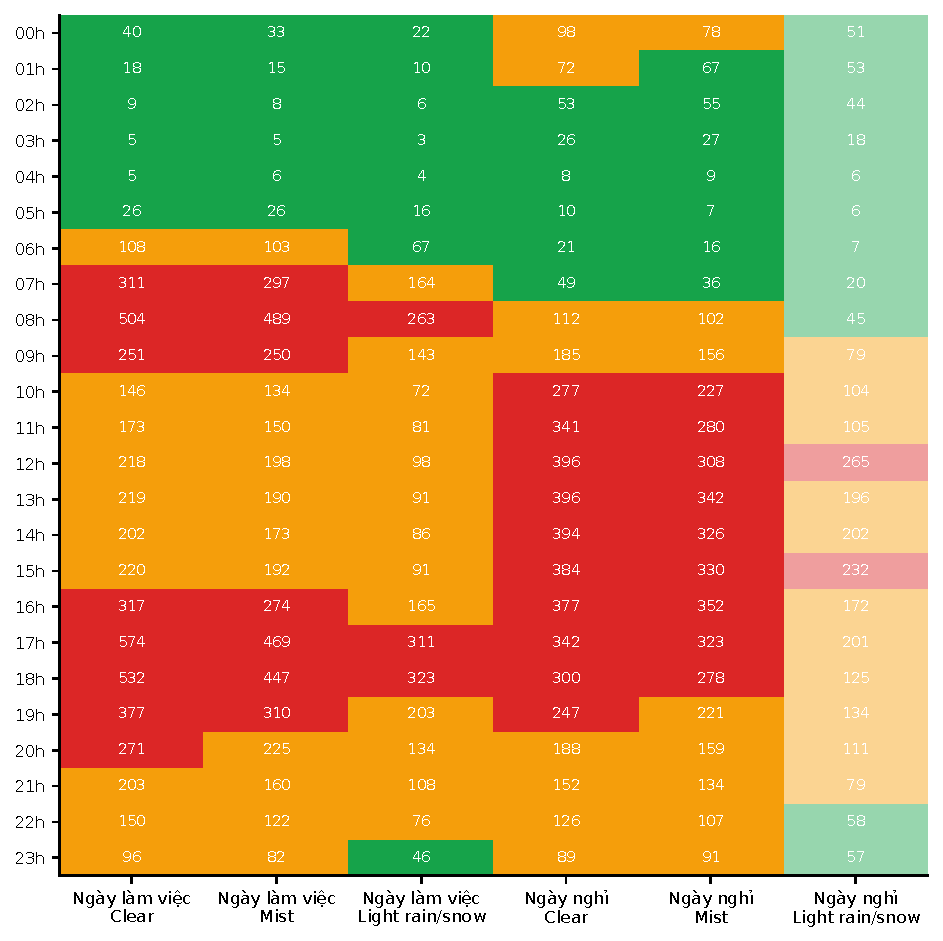
\includegraphics[width=0.82\textwidth]{figures/dss_matrix.pdf}
\caption{Ma trận phân loại giờ $\times$ loại ngày $\times$ thời tiết (số trong ô: lượt thuê TB/giờ; ô nhạt: dưới 30 giờ quan sát; bỏ cột mưa lớn do gần như không có dữ liệu)}
\label{fig:dss-matrix}
\end{figure}

\sect{Phân tích độ nhạy}\label{sec:dss-sensitivity}
Một đặc tính quan trọng của DSS là cho phép người dùng thay đổi giả định và quan sát ảnh hưởng (phân tích ``what-if''). Nhóm thử hai loại thay đổi trên tình huống ``ngày làm việc, trời quang'':

\begin{table}[H]
\centering
\caption{Phân tích độ nhạy của kết quả phân loại}
\label{tab:sensitivity}
\begin{tabularx}{\textwidth}{|p{4.6cm}|c|c|c|X|}
\hline
\textbf{Cấu hình} & \textbf{$\theta_L$} & \textbf{$\theta_H$} & \textbf{Số giờ Cao} & \textbf{Khung cảnh báo} \\ \hline
P33,3/P66,7, toàn bộ dữ liệu (mặc định) & 70 & 225 & 8 & 07--09h; 16--20h \\ \hline
P25/P75, toàn bộ dữ liệu & 40 & 281 & 6 & 07--08h; 16--19h \\ \hline
P33,3/P66,7, kỳ lịch sử 2012 & 98 & 284 & 8 & 07--09h; 16--20h \\ \hline
\end{tabularx}
\end{table}
Ngưỡng chặt hơn (P75) chỉ loại bớt giờ ``rìa'' của khung (9h và 20h), còn lõi cao điểm 7--8h và 16--19h không đổi. Khi chỉ dùng dữ liệu 2012 (nhu cầu cao hơn 2011 khoảng 65\%), ngưỡng tăng tương ứng nhưng các khung cảnh báo giữ nguyên. Kết luận: \textbf{các khung giờ ưu tiên là ổn định}, không phải hệ quả của việc chọn ngưỡng - tăng độ tin cậy của khuyến nghị.

\sect{Giao diện DSS}\label{sec:dss-ui}
Giao diện DSS nằm ở trang riêng ``Hỗ trợ quyết định'' của dashboard (\code{\#/dss}, Hình~\ref{fig:dash-dss-top}--\ref{fig:dash-dss-matrix}). Trang được thiết kế cho \textbf{người vận hành} (không cần hiểu thống kê) theo luồng đánh số từng bước, đi từ câu hỏi tới hành động:
\begin{enumerate}
    \item \textbf{Chọn tình huống sắp tới}: hai nhóm nút bấm lớn có mô tả ngắn - loại ngày (Ngày làm việc / Ngày nghỉ, \textit{hoặc} một / nhiều thứ cụ thể bằng hàng nút T2 \ldots{} CN bấm bật / tắt, có nút bỏ chọn; khi chọn từ hai thứ có thêm lựa chọn \textit{Từng thứ riêng} / \textit{Gộp thành 1 kế hoạch}) và thời tiết dự báo (Quang đãng, Sương mù, Mưa nhẹ, Mưa lớn). Kỳ lịch sử lấy từ bộ lọc dropdown Năm/Mùa (trang này chỉ hiện hai bộ lọc đó) và được nhắc lại bằng chữ ngay dưới các nút.
    \item \textbf{Kết luận}: một câu tóm tắt (ví dụ ``Có 2 khung giờ cao điểm. Cần chuẩn bị xong trước 06:00 và 15:00''), kèm số giờ ở mỗi mức, giờ đông nhất và nhãn nhóm khách của cả tình huống (ví dụ ``Nhiều khách vãng lai - 32,4\% lượt thuê, mức chung 18,8\%''). Khi tình huống hiếm gặp (đa số giờ không có hoặc có ít dữ liệu, như trời mưa lớn), hệ thống hiện cảnh báo \textit{không đủ dữ liệu để kết luận chắc chắn} thay vì đưa ra khuyến nghị gây hiểu nhầm.
    \item \textbf{Việc cần làm}: mỗi khung cảnh báo là một thẻ với mốc thời gian \textit{hoàn tất trước} nổi bật, khung giờ cao điểm, giờ đỉnh và lượt thuê trung bình, cùng nhãn nhóm khách của khung (kèm \% vãng lai) và khuyến nghị loại hỗ trợ tương ứng (Hình~\ref{fig:dash-dss-weekend}).
    \item \textbf{24 giờ trong ngày}: dải 24 ô tô màu theo mức để nhìn nhanh cả ngày, biểu đồ cột với hai đường ngưỡng, và ba thẻ giải thích ngưỡng cùng khuyến nghị của từng mức.
    \item \textbf{Nhóm khách cần phục vụ} (Hình~\ref{fig:dash-dss-users}): biểu đồ cột chồng lượt thuê của khách đăng ký và vãng lai theo giờ, dải 24 ô tô màu theo nhóm khách, giải thích mốc phân nhóm (tính theo tỷ lệ chung của kỳ) và ba thẻ khuyến nghị theo nhóm khách.
\end{enumerate}
Ở chế độ \textit{Từng thứ riêng} (Hình~\ref{fig:dash-dss-compare}), các bước trên được trình bày dạng so sánh: mỗi thứ một thẻ kết luận; việc cần làm nhóm theo từng thứ; các dải 24 ô xếp chồng (mỗi thứ một hàng) cùng biểu đồ đường, mỗi đường là một thứ; dải nhóm khách cũng xếp theo từng thứ; phần chi tiết có bảng so sánh từng giờ giữa các thứ.
Phần dành cho người phân tích được \textbf{thu gọn mặc định} (mở khi cần): bảng chi tiết từng giờ (nhu cầu, hệ số so với trung bình, số giờ quan sát, tỷ lệ khách vãng lai, nhóm khách, mức, khuyến nghị); giải thích cách xác định ngưỡng kèm bảng khảo sát phân phối và lựa chọn cách chia ngưỡng (phân tích độ nhạy); ma trận phân loại cho mọi tình huống.

\begin{figure}[H]
\centering
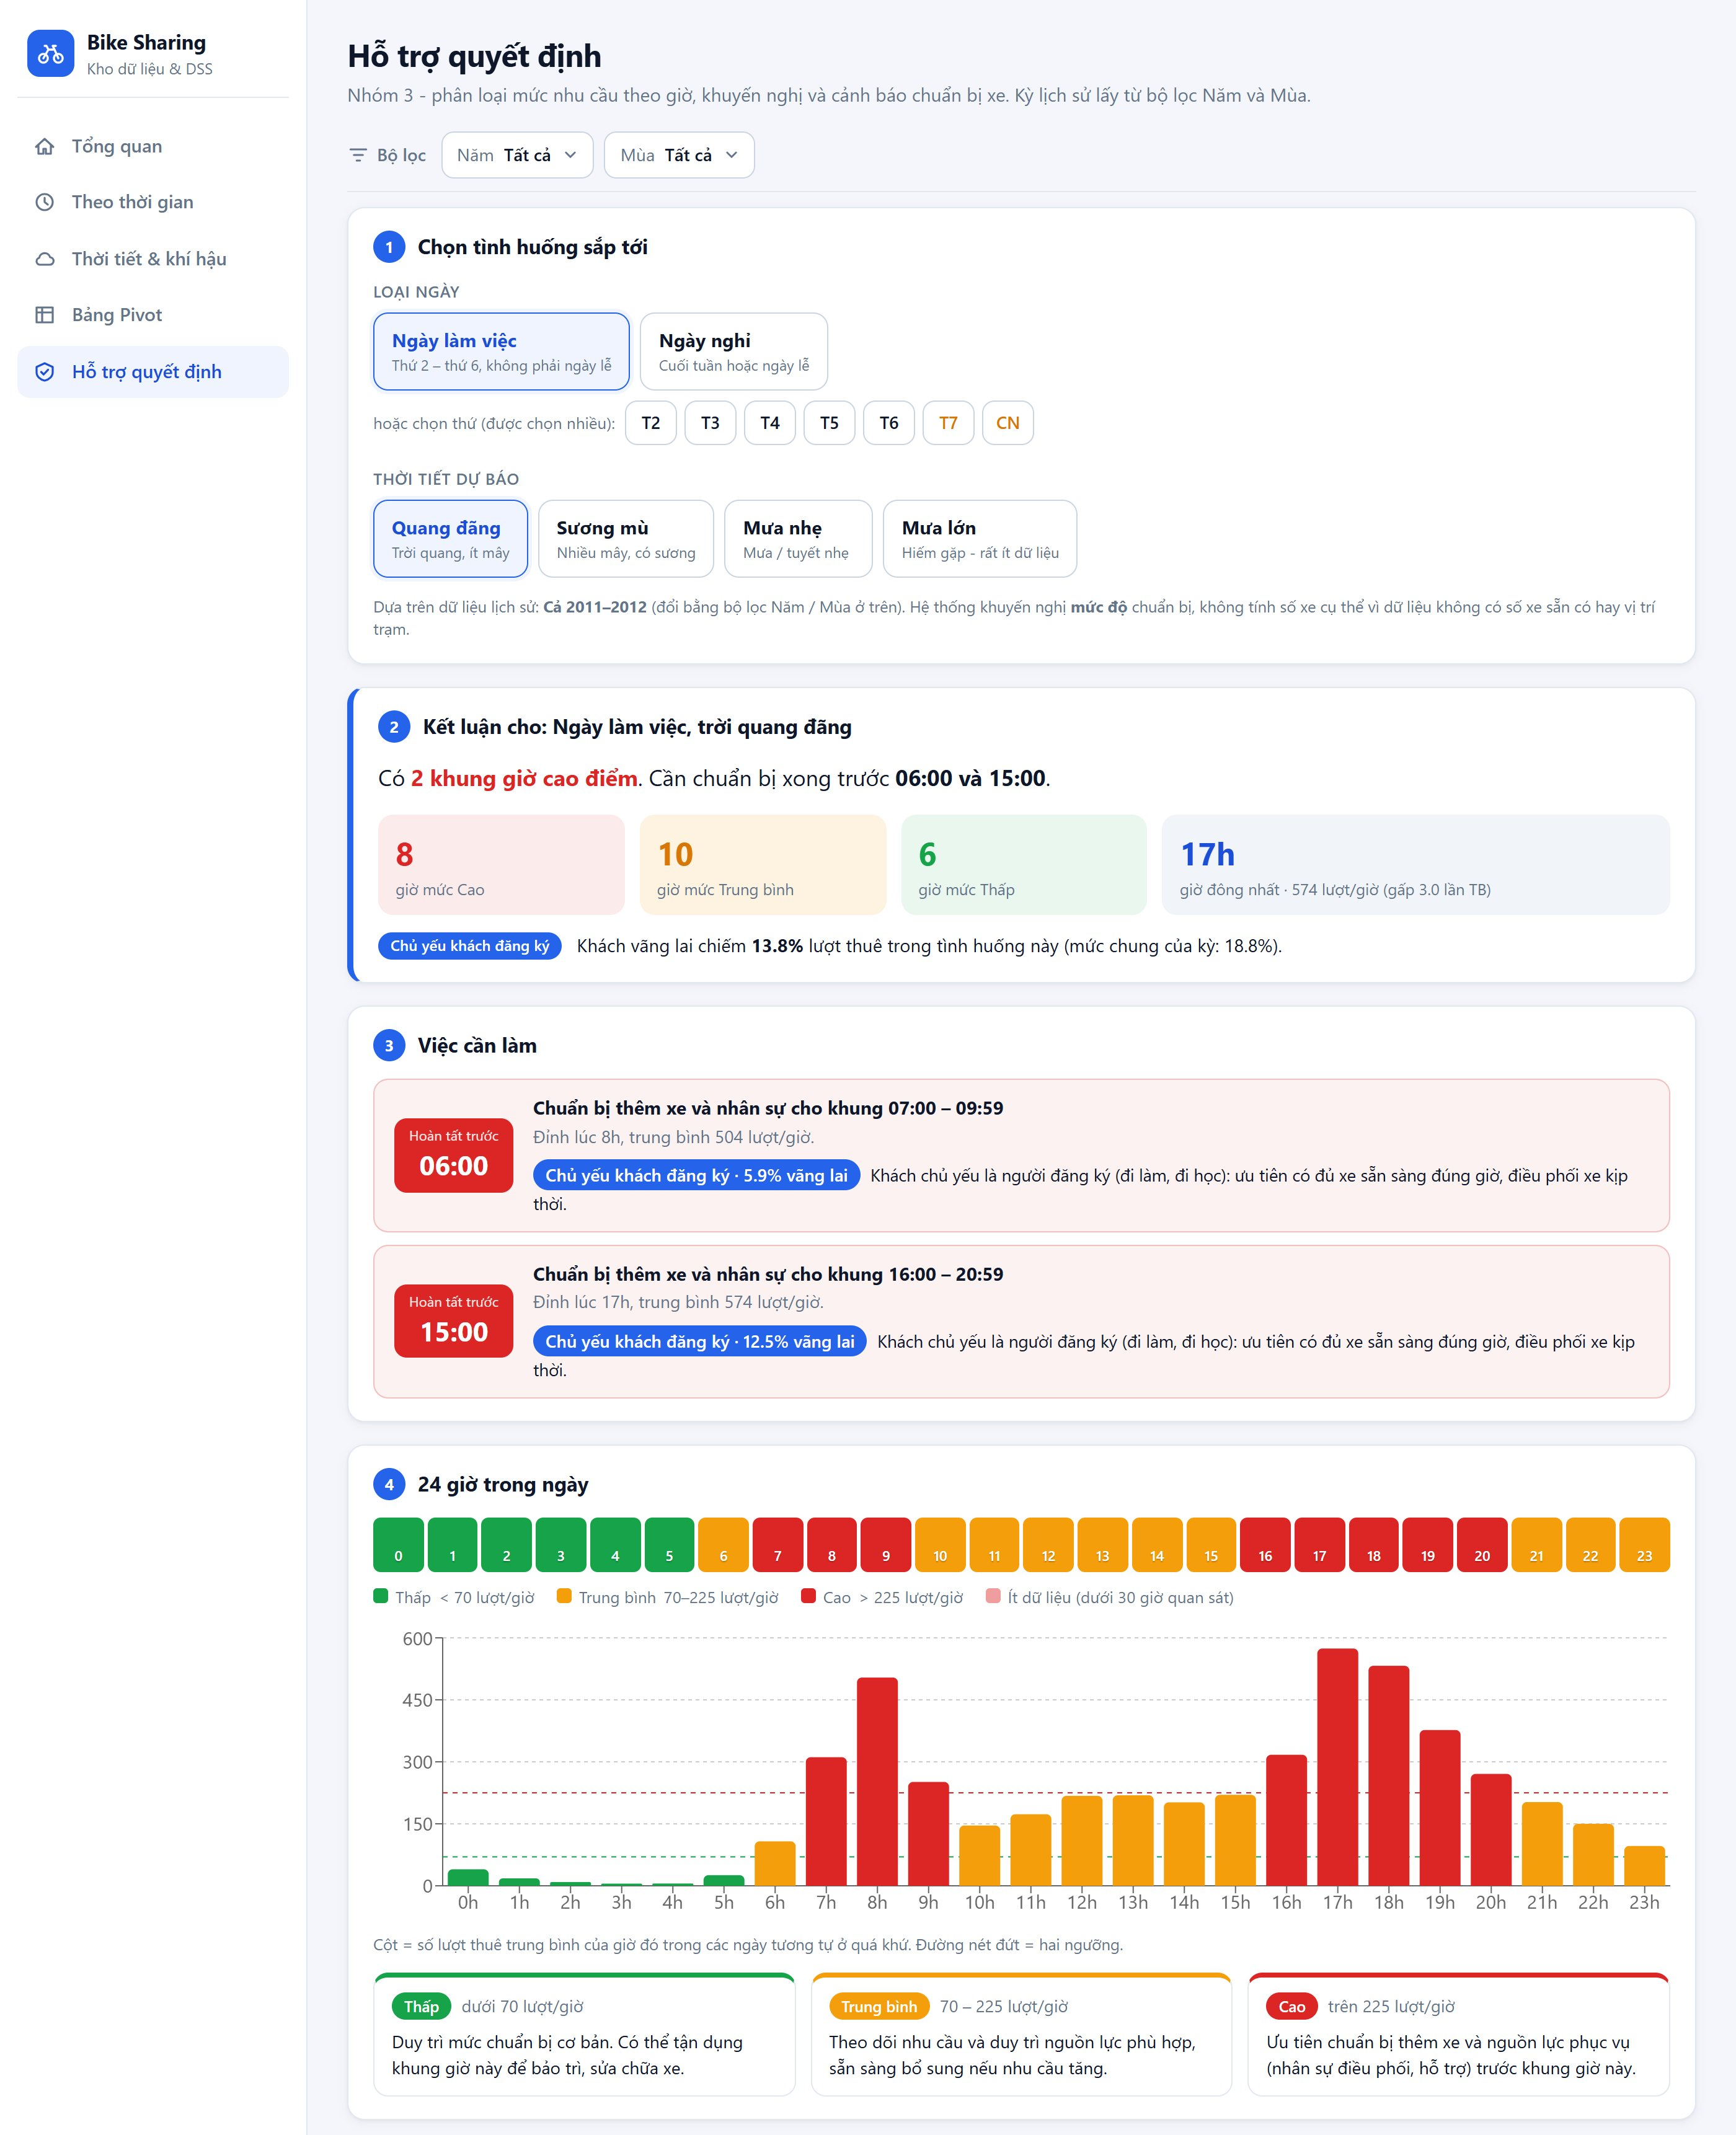
\includegraphics[width=0.85\textwidth]{figures/dash_dss_top.jpg}
\caption{Giao diện DSS: chọn tình huống, kết luận, việc cần làm và mức nhu cầu 24 giờ (ngày làm việc, trời quang đãng)}
\label{fig:dash-dss-top}
\end{figure}

\begin{figure}[H]
\centering
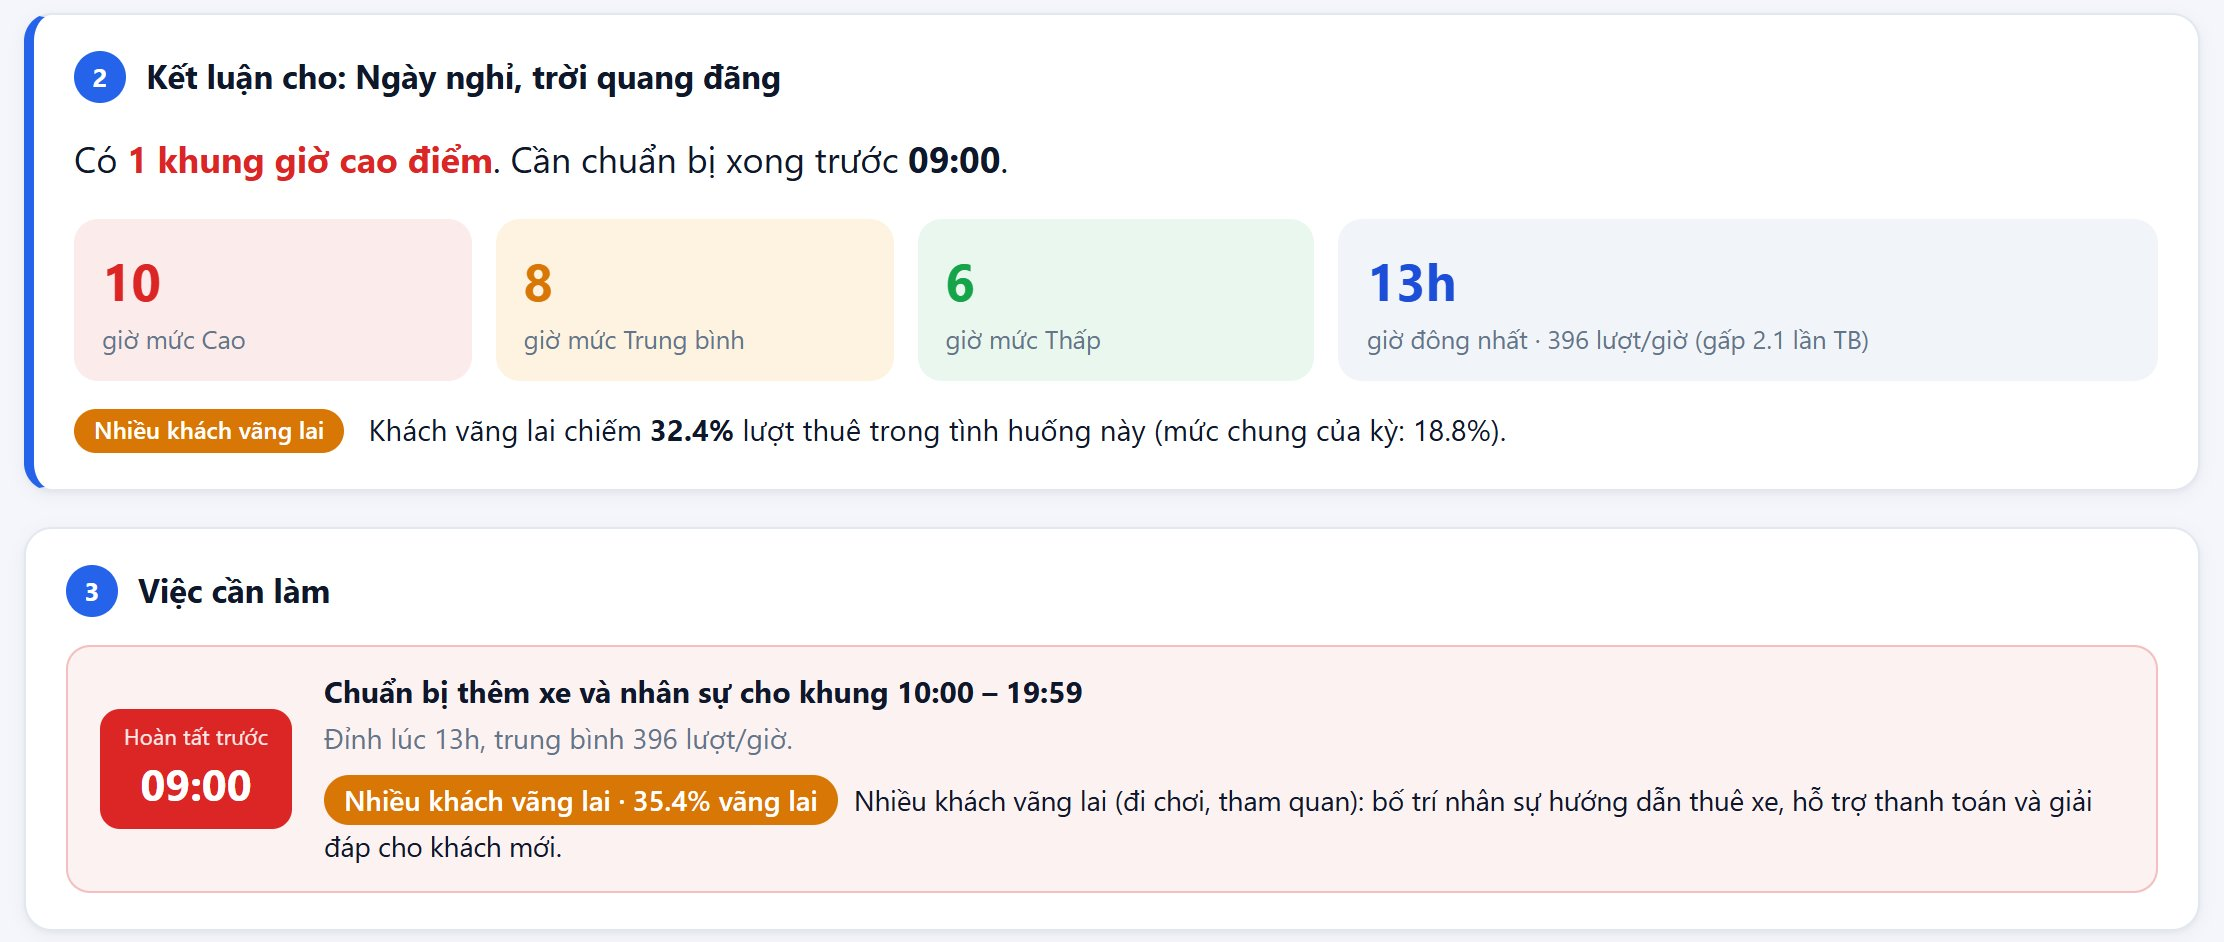
\includegraphics[width=0.9\textwidth]{figures/dash_dss_weekend.jpg}
\caption{Giao diện DSS với tình huống ngày nghỉ, trời quang đãng: kết luận và việc cần làm kèm nhóm khách (nhiều khách vãng lai)}
\label{fig:dash-dss-weekend}
\end{figure}

\begin{figure}[H]
\centering
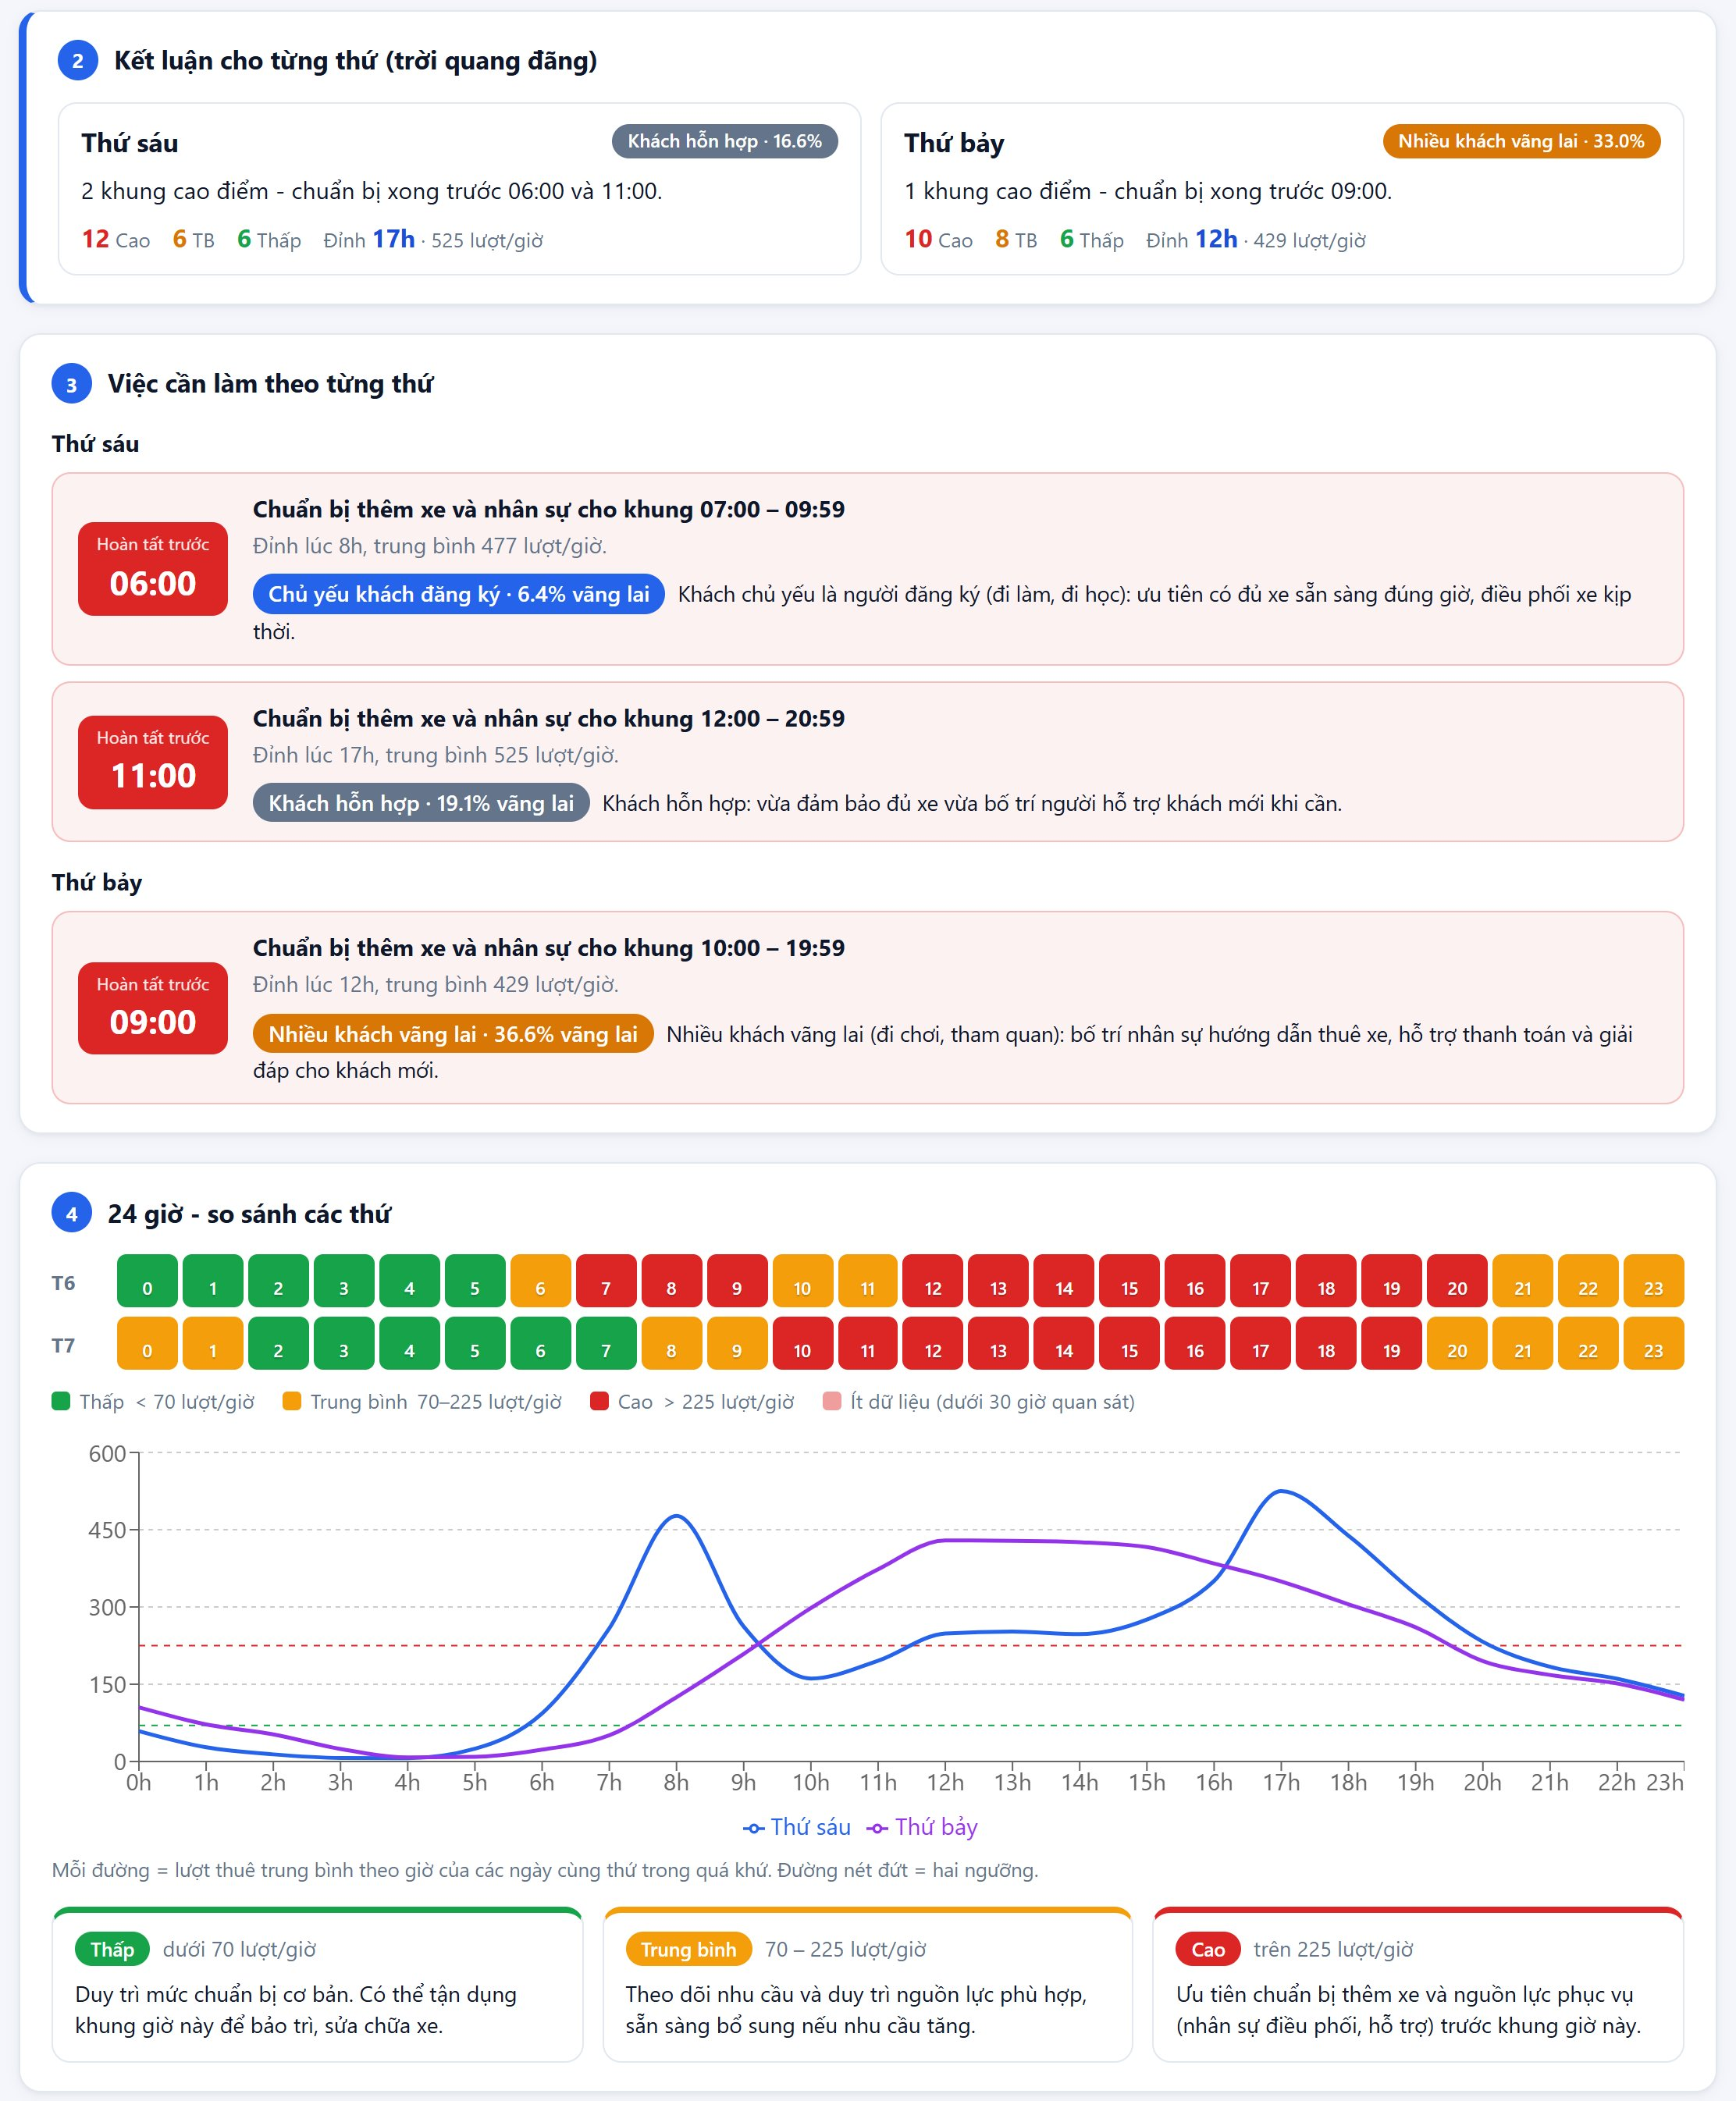
\includegraphics[width=0.8\textwidth]{figures/dash_dss_compare.jpg}
\caption{Giao diện DSS khi chọn thứ sáu và thứ bảy (chế độ \textit{Từng thứ riêng}): kết luận, việc cần làm và mức nhu cầu 24 giờ của từng thứ}
\label{fig:dash-dss-compare}
\end{figure}

\begin{figure}[H]
\centering
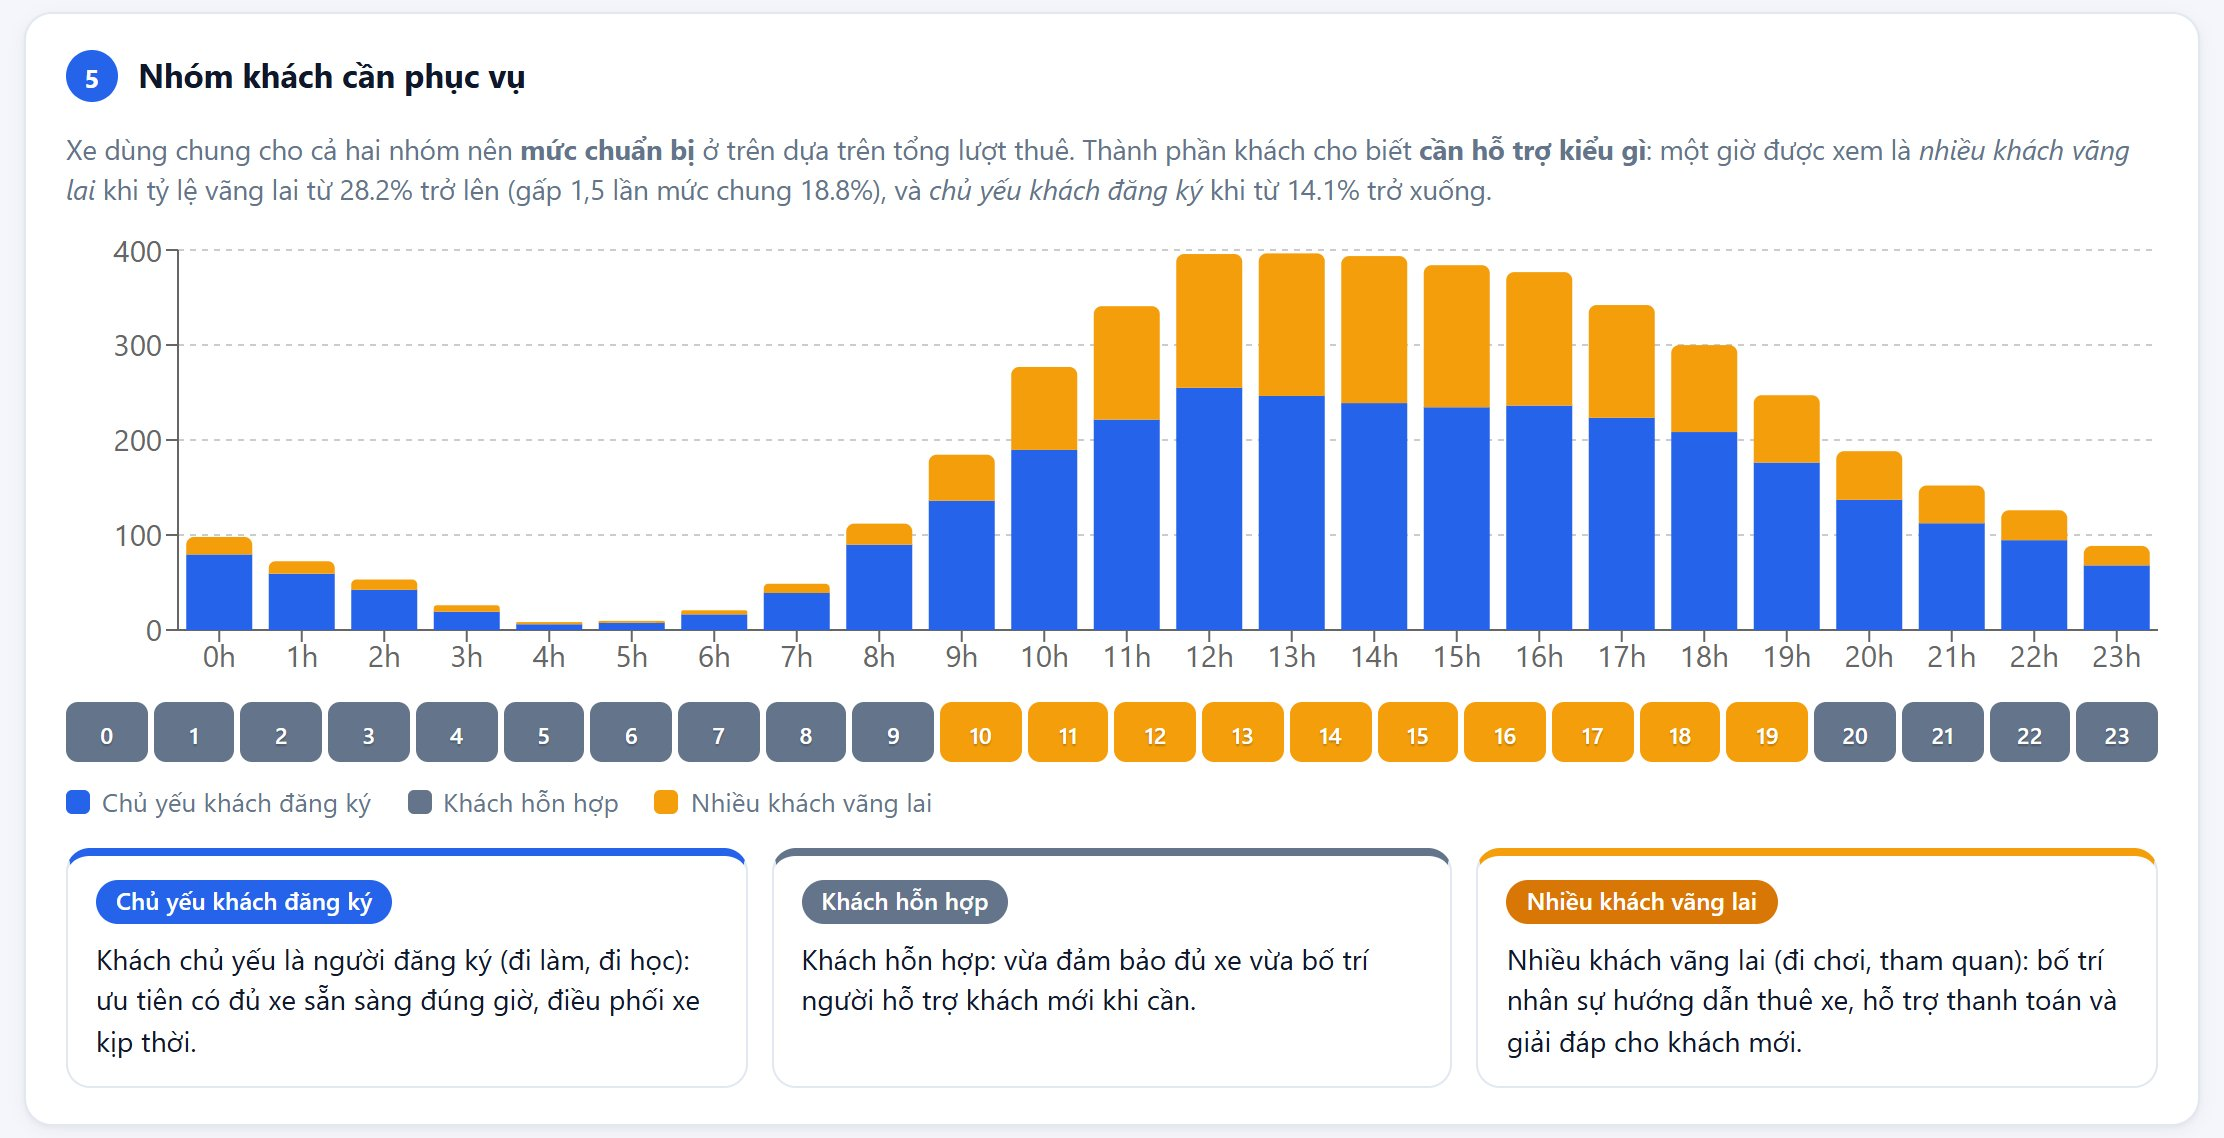
\includegraphics[width=0.9\textwidth]{figures/dash_dss_users.jpg}
\caption{Giao diện DSS: thành phần khách theo giờ và khuyến nghị theo nhóm khách (ngày nghỉ, trời quang đãng)}
\label{fig:dash-dss-users}
\end{figure}

\begin{figure}[H]
\centering
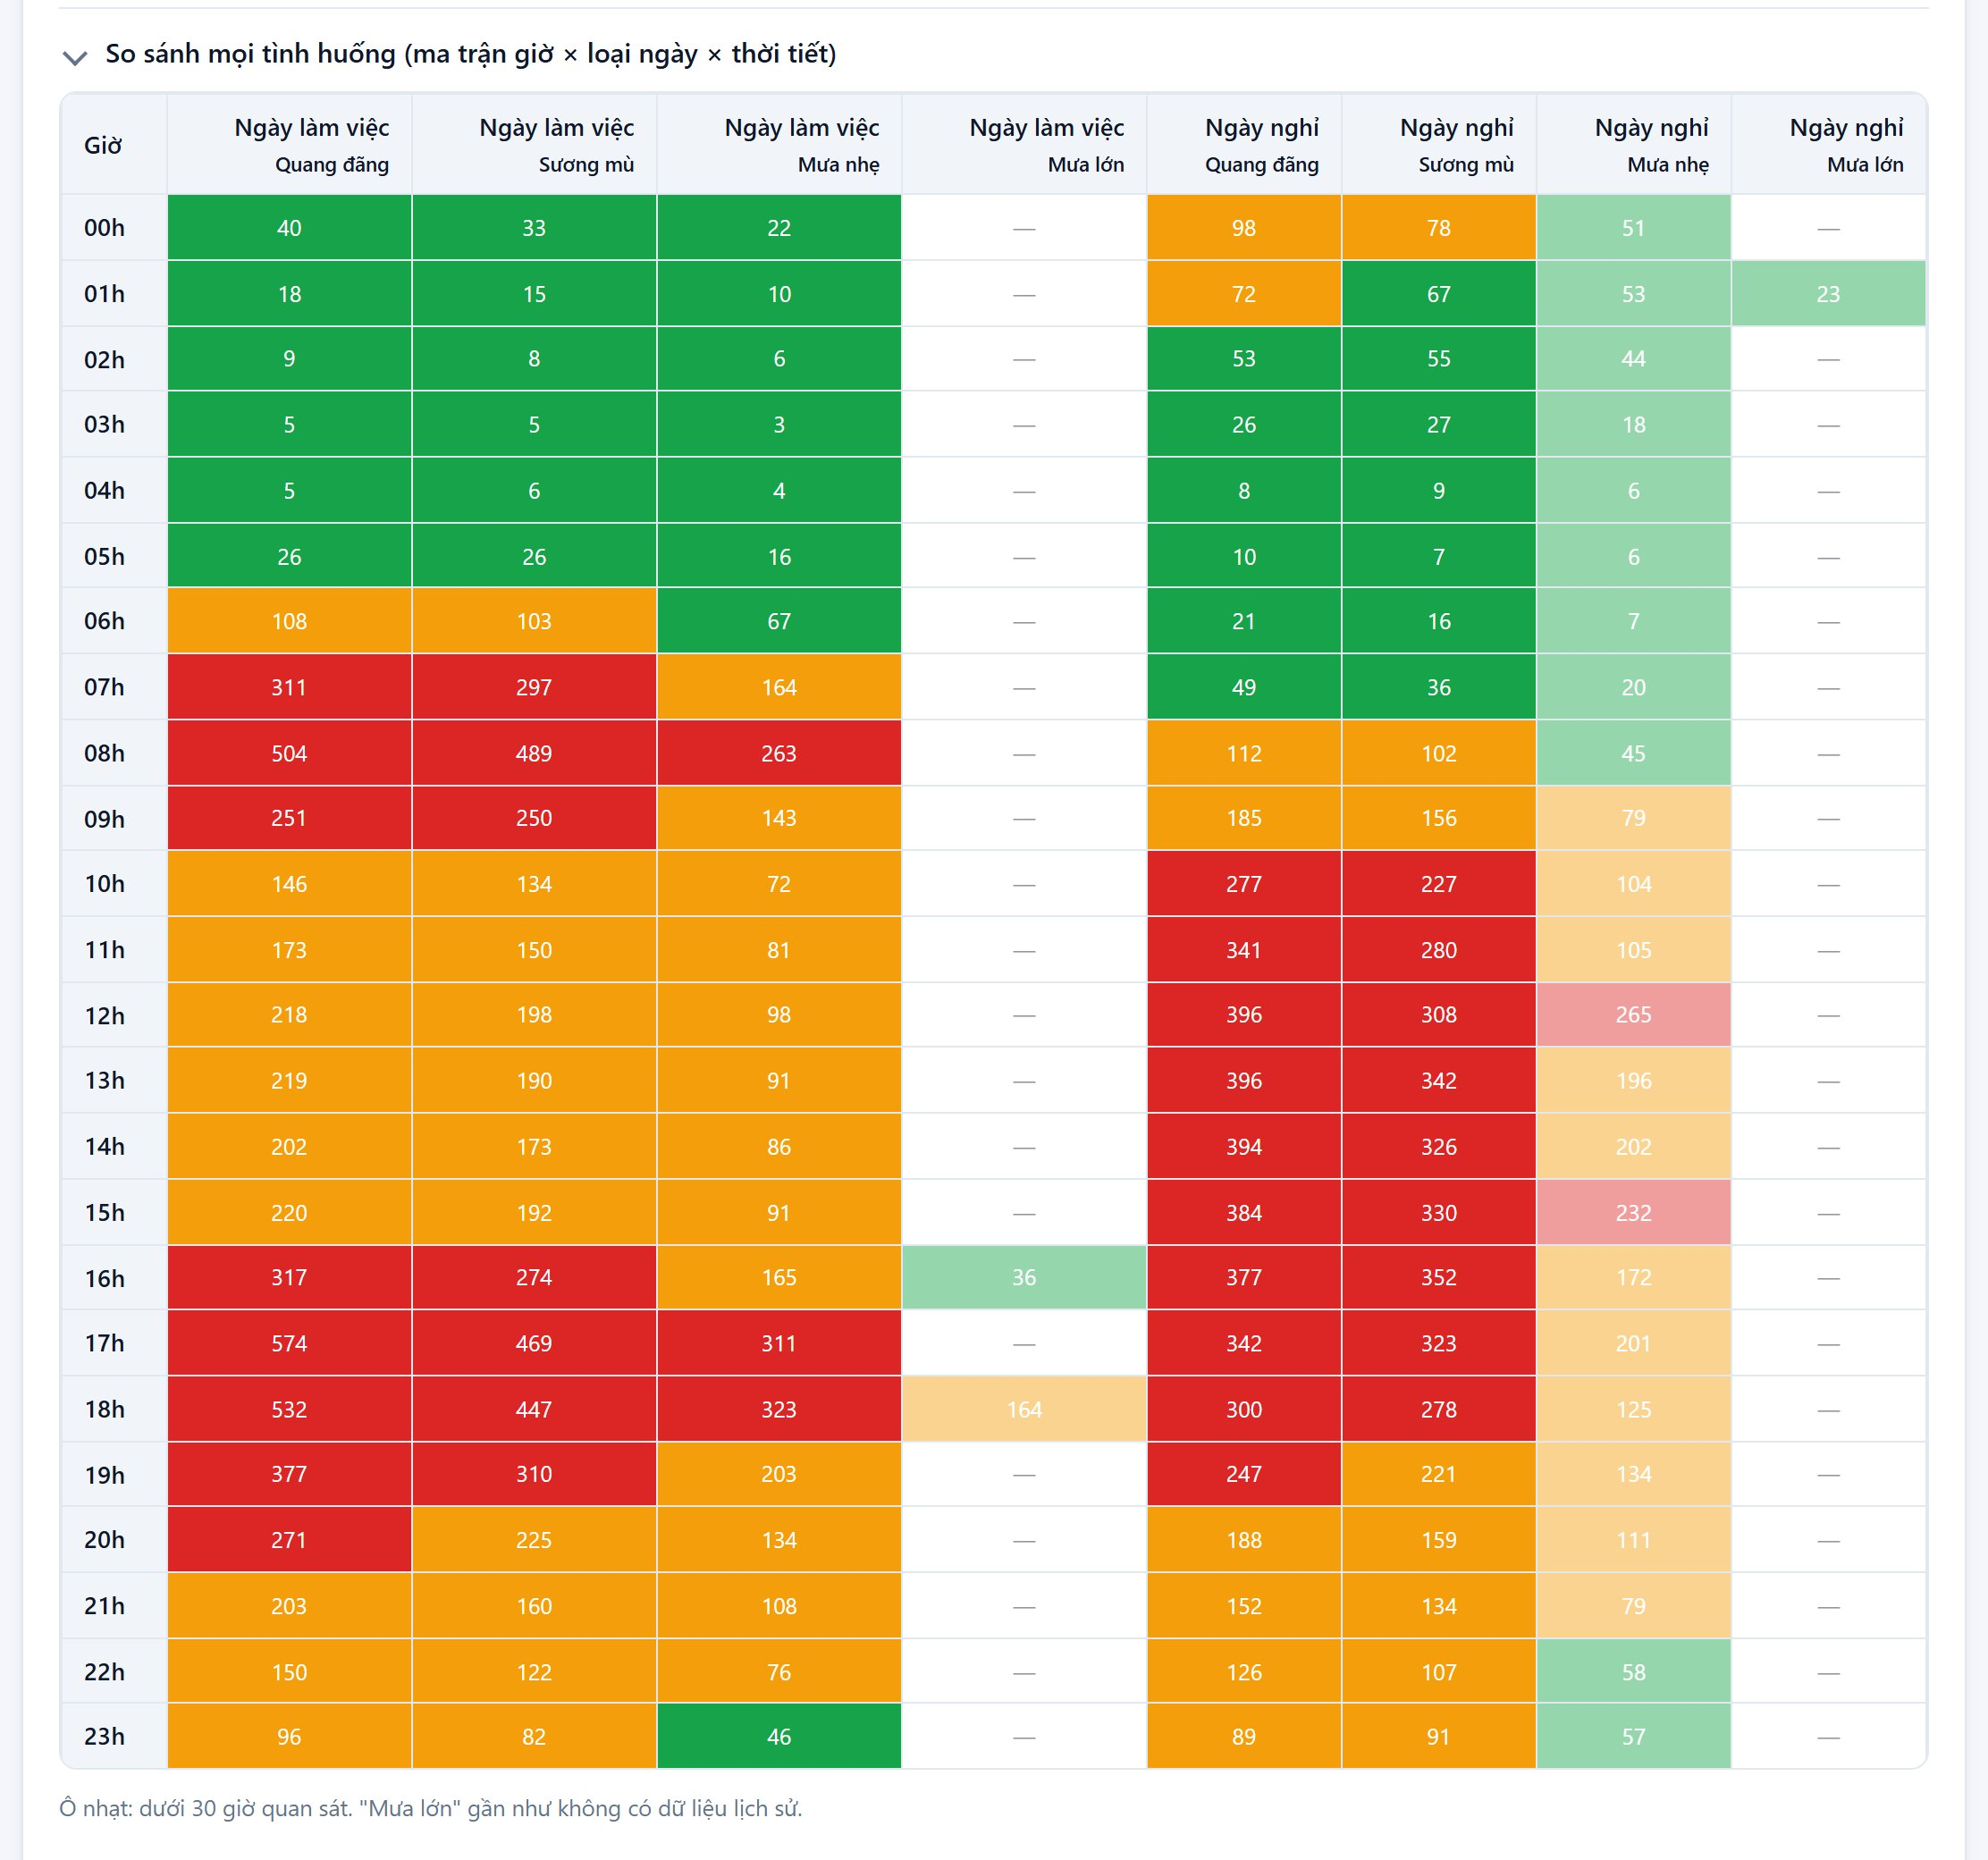
\includegraphics[width=0.92\textwidth]{figures/dash_dss_matrix.jpg}
\caption{Giao diện DSS: ma trận phân loại giờ $\times$ loại ngày $\times$ thời tiết (phần chi tiết, mở khi cần)}
\label{fig:dash-dss-matrix}
\end{figure}
